\section{Evaluation}
\label{sec:evaluation}

All the results presented in this sections are obtained with a test set containing the examples from $3001$ to $5000$.

\subsection{Training Error}
\begin{figure}[t]
	\centering
	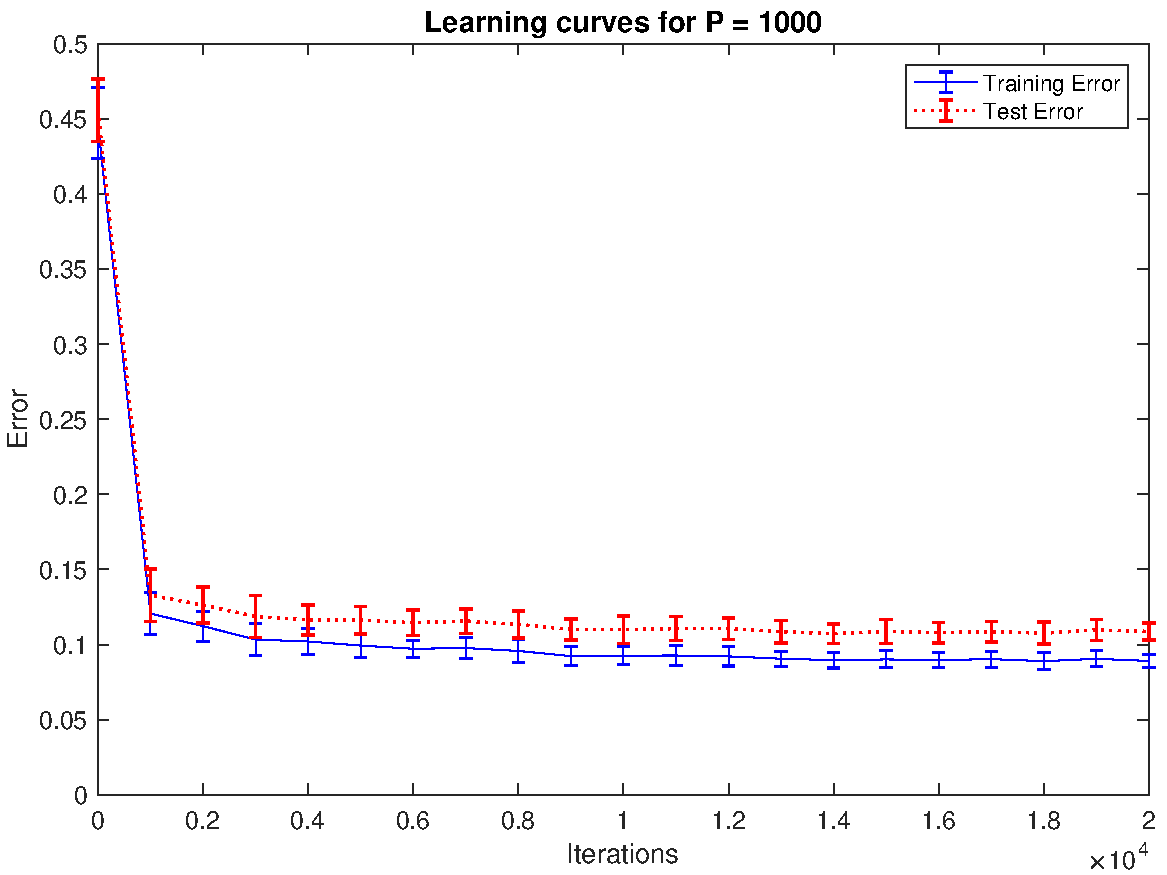
\includegraphics[width=\columnwidth]{figures/error}
    \caption{Training and test error of the network for $P = 1000$.}
	\label{fig:training_error}
\end{figure}

\cref{fig:training_error} shows the train and test error for the network trained using Stochastic Gradient Descent on the first $1000$ examples.
Both the train error and test error drop very quickly during approximately the first $1000$ iterations, then remain almost constant for the rest of the training.
The test error is slightly bigger than the train error:
at the end of the training, the train error is around $0.10$ and the test error around $0.12$.
Since the test error never increases, the model does not seem to overfit the training data.

\subsection{Learned Weights}

\subsection{Training Dataset}

\subsection{Training Policy}
The learning rate is well known to influence the number of iterations the network needs to minimize
its cost function. It is nevertheless true that a high value for this variable causes the network to
be unstable since it learns the same amount of information from all the data that are presented to it (no matters the number of iterations).
For this reason we decided to implement some different schedulers for the learning rate able to change its
value over time and not to leave it fixed.

The implemented learning rate policies are: \textit{fixed}, \textit{step}, \textit{exponential} and \textit{triangular}.
In the figure below \cref{fig:learning_rates_policies} it's possible to take a look at the way they change the value of the learning rate over time (i.e. iterations).


\begin{figure}
	\centering
	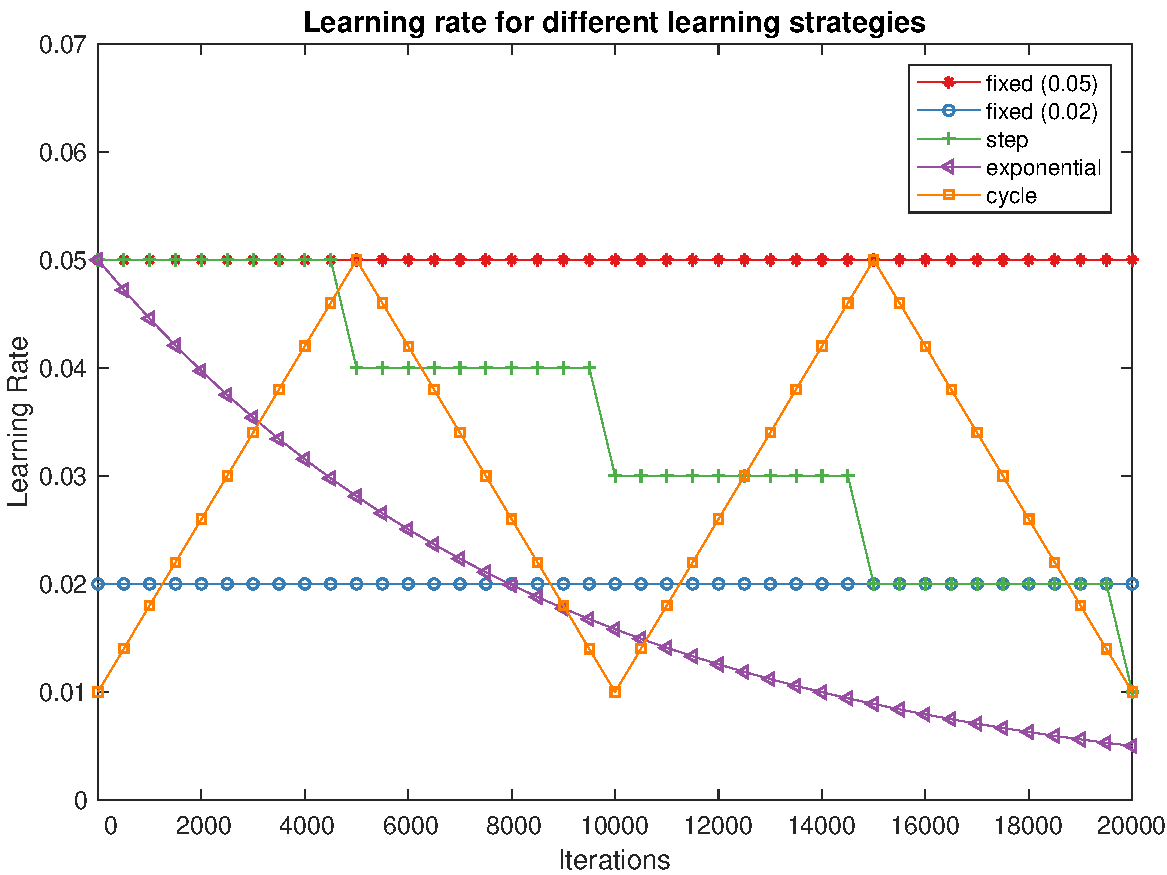
\includegraphics[width=\columnwidth]{figures/learning_rates}
	\caption{Learning rate evolution over iterations for different learning rate policies.}
	\label{fig:learning_rates_policies}
\end{figure}

\begin{figure}
	\centering
	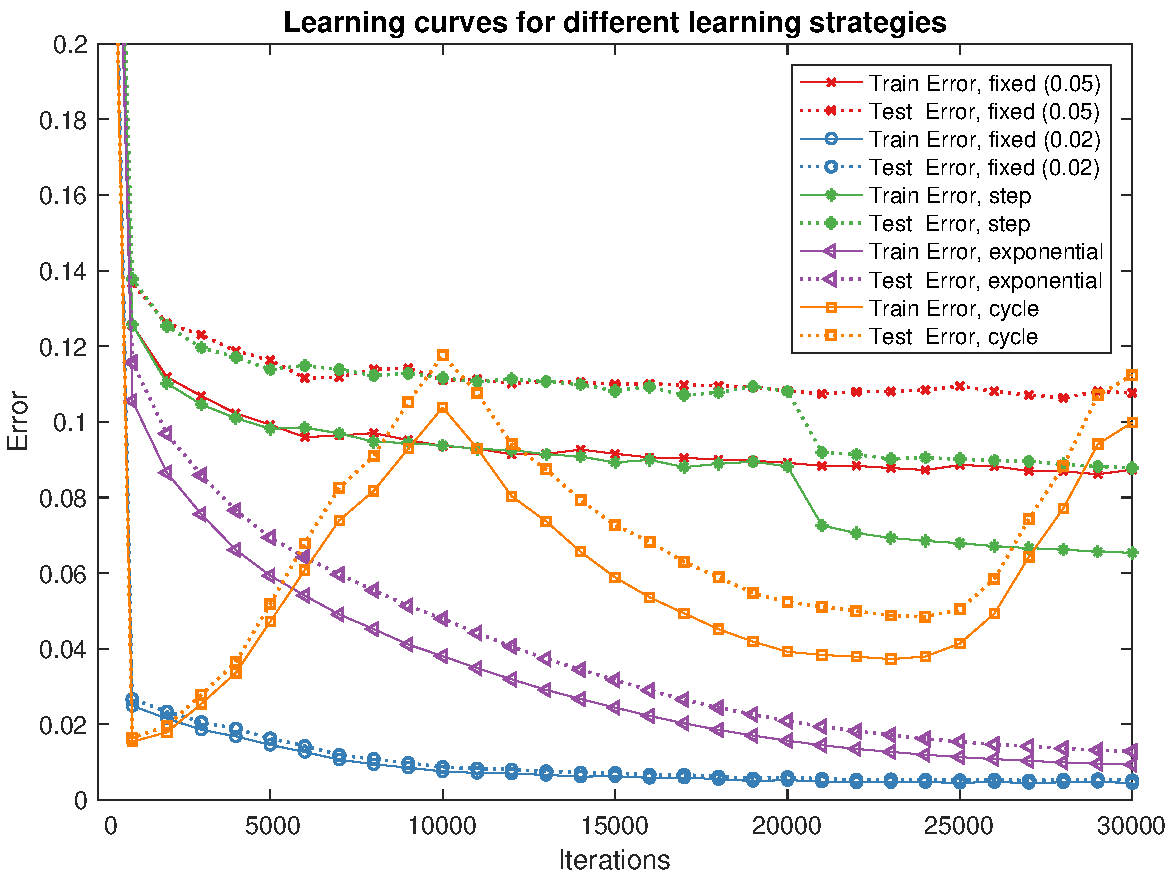
\includegraphics[width=\columnwidth]{figures/error_strategies.pdf}
	\caption{Training and test error for different learning rate policies.}
	\label{fig:lrp_training_error}
\end{figure}
